\documentclass[../../szobeli.tex]{subfiles}

\begin{document}

\begin{center}
    \noindent\fbox{%
    	\parbox{160mm}{
			\textbf{Lineáris egyenletrendszer, kibővített együtthatómátrix, elemi sorekvivalens átalakítás} és \underline{kapcsolata a megoldásokkal}. \textbf{LA és RLA mátrix, vezéregyes, megoldás leolvasása RLA mátrix esetén}. Tilos sor, kötött változó, szabad paraméter, \underline{ezek jelentése a megoldás/megoldhatóság szempontjából.} \textbf{Gauss-elimináció}, \underline{összefüggés az egyértelmű megoldhatóság, az egynletek és ismeretlenek száma között}.
        }
    }
\end{center}

    \begin{itemize}
        \item \textbf{Lineáris egyenletrendszer}
        
            \textcolor{blue}{\textbf{Def:}} \textcolor{red}{Lineáris egyenlet:} Ismeretlenek konstansszorosainak összege konstans. \textcolor{red}{Lineáris egyenletrendszer:} Véges sok lineáris egyenlet. \textcolor{red}{Megoldás:} Olyan érték adás, ami minden egyenletet igazzá tesz.

        \item \textbf{Kibővített együtthatómátrix} 
        
            \textcolor{blue}{\textbf{Def:}} \textcolor{red}{Lineáris egyenletrendszer kibővített együtthatómátrixa:} a sorok az egyenletek, az oszlopok az ismeretleneknek ill. az egyenletek jobb oldalainak felelnek meg, az egyes mezőkben pedig a megfelelő együttható ill. jobb oldali konstans áll. 
            
        \item \textbf{Elemi sorekvivalens átalakítás} \underline{és kapcsolata a megoldásokkal} 
        
            \textcolor{green}{\textbf{Biz:}} Minden ESÁ előtti megoldás megoldás marad az ESÁ után is. Minen ESÁ fordítottja megkapható ESÁ-ok egymásutánjaként is. Ezért minden ESÁ utáni megoldás megoldja az ESÁ előtti előtti rendszert is. 

            \textcolor{blue}{\textbf{Megj:}} A kibővített együtthatómátrix a lineáris egyenletrendszer felírásának egy tömör módja: elkerüljük vele a műveleti- és egyenlőségjelekkel piszmogást, mégis telejesen áttekinthető módon tartalmaz minden lényeges információt.

            \textcolor{violet}{\textbf{Megoldás módszere}} Ekvivalens átalakításokat végzünk. Ezek során a megoldások halmaza nem változik. Konkrétan: egyenleteket felcserélünk, egyenletet nemnullával vigigszorzunk ill. az $i$-dik egyenletet kicseréljük az $i$-dik és $j$-dik egyenletek összegére.
            
            \textcolor{blue}{\textbf{Def:}} A kibővített együtthatómátrix \textcolor{red}{elemi sorekvivalens átalakítása (ESÁ)}: (1) sorcsere, (2) sor nemnulla konstanssal végigszorzása, (3) az $i$-dik sor helyettesítése az $i$-dik és $j$-dik sorok (koordiántánkénti) összegével (az $i$-dik sor helyettesítése az $i$-dik sor és a $j$-dik sor konstansszorosának összegével, csupa 0 sor hozzáadása/elhagyása).

        \item \textbf{LA és RLA mátrix, vezéregyes}
        
            \textcolor{blue}{\textbf{Def:}} Az $M$ mártix \textcolor{red}{lépcsős alakú} (\textcolor{red}{LA}), ha 
            
            (1) minden sor első nemnulla eleme 1-es (ú.n. \textcolor{red}{vezér 1-es}, avagy \textcolor{red}{v1}) 

            (2) minden v1 feletti sorban van ettől a v1-től balra eső másik v1.

            Az $M$ mátrix \textcolor{red}{redukált lépcsős alakú} (\textcolor{red}{RLA}), ha 

            (3) $M$ LA és (2) $M$-ben minden v1 felett csak nullák állnak. 

            \textcolor{violet}{\textbf{Példa:}} LA mátrix \hspace{30mm} RLA mátrix

            $ \begin{pmatrix}
                \textcolor{red}{1} & 3 & -2 & 0 & 1 & 1 & 7 \\
                0 & 0 & \textcolor{red}{1} & 2 & 0 & 5 & -2 \\
                0 & 0 & 0 & 0 & \textcolor{red}{1} & 1 & -1 \\
                0 & 0 & 0 & 0 & 0 & \textcolor{red}{1} & 5 \\
                0 & 0 & 0 & 0 & 0 & 0 & 0 
            \end{pmatrix}  $ ill. 
            $ \begin{pmatrix}
                0 & \textcolor{red}{1} & 0 & -2 & 0 & 1 & 0 \\
                0 & 0 & \textcolor{red}{1} & 2 & 0 & 5 & 0 \\
                0 & 0 & 0 & 0 & \textcolor{red}{1} & 1 & 0 \\
                0 & 0 & 0 & 0 & 0 & 0 & \textcolor{red}{1} \\
                0 & 0 & 0 & 0 & 0 & 0 & 0 
                \end{pmatrix}  $

        \item \textbf{Megoldás leolvasása RLA mátrix esetén}
        
            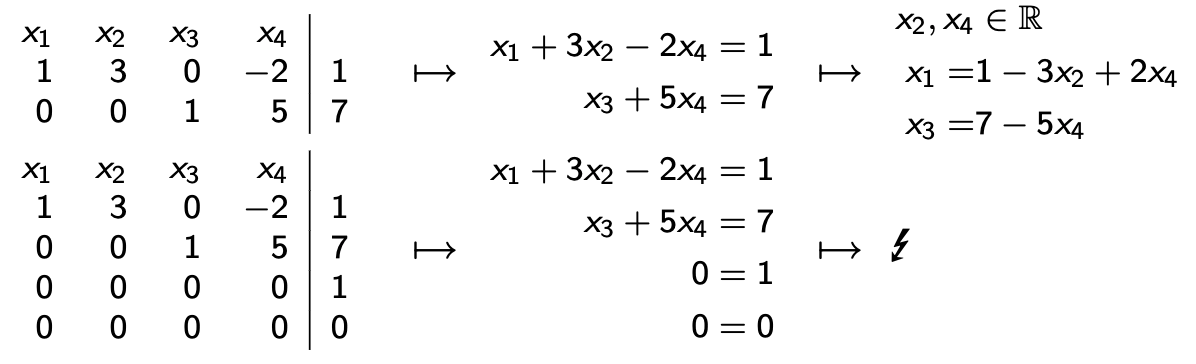
\includegraphics[scale=0.38]{img/1.png}

        \item Tilos sor
        
            \textcolor{blue}{\textbf{Def:}} Kibővített együtthatómátrix \textcolor{red}{tilos sora}: $0 \dots 0 | x$ alakú sor, ha $x \neq 0$.

        \item Kötött változó és szabad paraméter
        
            \textcolor{blue}{\textbf{Def:}} A RLA kibővített együtthatómátrix v1-hez tartozó változója \textcolor{red}{kötött}m a többi változó (amihez nem tartozik v1) \textcolor{red}{szabad} (vagy \textcolor{red}{szabad paraméter}). 

            \textcolor{orange}{\textbf{Megf:}} Ha kibővített együtthatómátrix RLA, akkor (1) minden sor vagy a v1-hez tartozó változó értékadása, vagy tilos sor, vagy csupa 0 sor.

            (2) Ha van tilos sor, akkor nincs megoldás. 

            (3) Ha nincs tilos sor, a szabad paraméterek tetszőleges, értékadásához egyértelmű megoldás tartozik.

            \textcolor{orange}{\textbf{Megf:}} A lineáris egyenletrendszer megoldása tekinthető úgy, hogy a lineáris egyenletrendszeregy RLA kibővített együtthatómátrixal van megadva.

            \textcolor{red}{\textbf{Cél:}} Olyan eljárás, ami ESÁ-okkal tetszőleges mátrixot RLA-vá alakít.

        \item \textbf{Gauss elimináció}
        
            \textcolor{blue}{\textbf{Gauss-elimináció:}} 
            
            \underline{Input:} $M \in \mathbb{R}^{n \times k}$ mátrix.

            \underline{Output:} Egy $M$-ből ESÁ-okkal kapható $M' \in \mathbb{R}^{n \times k}$ LA mátrix.

            \underline{Működés:} Az algoritmus fázisokból áll. Az $i$-dik fázisban keresünk egy nemnulla elemet az ($i-1$)-dik sor alatt a lehető legkisebb sorszámú oszlopban. Ha nincs ilyen elem, az algoritmus véget ér. Sorcserével ezt a nemnulla elemet az $i$-dik sorban visszük. Az $i$-dik sor konstanssal szorzásával ezt az elemet v1-sé alakítjuk. Az $i$-dik sor alatti sorokhoz az $i$-dik sor konstansszorosát hozzáadva kinullázuk a kapott v1 alatti elemeket.

        \item \underline{összefüggés az egyértelmű megoldhatóság, az egynletek és ismeretlenek száma között}
        
            \textcolor{blue}{\textbf{Megj:}} (1) A Gauss-elimináció outputja LA. Az RLA-hoz további lépésekre van szükség: minden v1 felett kinullázhatók az elemek, ha a v1 sorának konstansszorosait a v1 feletti sorokhoz adjuk. 

            (2) Ha csupán LA (vagy RLA) a cél, eltérhetünk a Gauss-eliminációtól, feltéve, hogy ESÁ-okkal dolgozunk.

            (3) A Gauss-elimináció megvalósítható rekurzív algoritmusként is. 

            A GE($M$) (az $M$ mátrixot lépcsős alakra hozó eljárás):

            \fbox{1.} Ha $M$ első oszlopa csupa 0, akkor $M'$ az első oszlop törlésével keletkező mátrix. Output: GE($M'$) elé írunk egy csupa 0 oszlopot.

            \fbox{2.} Ha $M$ első oszlopa tartalmaz nemnulla elemet, sorcserével és az első sor konstanssal szorzásával az első sor első elemét v1-sé tesszük, majd a v1 alatti elemeket ESÁ-okkal kinullázzuk. Legyen $M'$ az első sor és első oszlop törlésével keletkező mátrix. Output: GE($M'$) elé írunk egy csupa 0 oszlopot és az így kapott mátrix fölé a korábban törölt első sort.

            \begin{enumerate}
                \item Lineáris egyenletrendszer kibővített együtthatómátrixként is magadható.
                \item ESÁ nem változtat a megoldásokon.
                \item ESÁ-okkal elérhető a RLA.
                \item A RLA-ból azonnal adódik a megoldás \begin{itemize}
                    \item Ha az utolsó oszlopban van v1, akkor nincs megoldás.
                    \item Ha az utolsó kivételével minden oszlopban van v1, akkor egyetlen megoldás van.
                    \item Ha az utolsón kívül más oszlopban nincs v1, akkor van szabad paraméter, így végtelen sok különböző megoldás van.
                \end{itemize}
            \end{enumerate}

            \textcolor{orange}{\textbf{Köv:}} Ha a lineáris egyenletrendszernek pontosan egy megoldása van, akkor legalább annyi egyenlet van, mint ahány ismeretlen.

            \textcolor{green}{\textbf{Biz:}} Az RLA-ra hozás után nincs szabad paraméter, tehát minden változóhoz tartozik v1. Ezért a kibővített együtthatómátrixnak legalább annyi sora van, mint a változók száma.

            \textcolor{blue}{\textbf{Megj:}} A fenti következmény fordított irányban nem igaz, és lényegében nincs más összefüggés az egyértelmű megoldhatóság, az ismeretlenek és egyneletek száma között.
        
    \end{itemize}

\textcolor{red}{}

    
\end{document}